\chapter{Authentication Module}
\minitoc
\clearpage
\section{Introduction}
The authentication module controls secure access and verifies user identity. It manages registration, login, administrator approval, and an extra OTP email check for Admin login.

This module is designed to:
\begin{itemize}[noitemsep]
    \item Protect sensitive data.
    \item Restrict access to authorized users only.
    \item Enforce role-based access (Admin, HR, Project Manager).
\end{itemize}

The authentication flow adds one extra validation step: newly registered users must be approved by an administrator before they can access the system.

\section{Sprint Backlog}
During this sprint, we selected and implemented the following user stories:

\begin{center}
\renewcommand{\arraystretch}{1.2}
\begin{tabular}{|l|>{\raggedright\arraybackslash}p{9.2cm}|l|}
\hline
\textbf{ID} & \textbf{User Story} & \textbf{Priority} \\
\hline
US1 & As a user, I want to log in using my email and password. & High \\
\hline
US2 & As a HR/Project Manager, I want to create an account. & High \\
\hline
US3 & As an admin, I want to approve user accounts. & High \\
\hline
US4 & As an admin, I want to receive an OTP code by email during login for extra verification. & High \\
\hline
US5 & As a user, I want to receive an email after approval. & Medium \\
\hline
US6 & As a system, I must prevent unapproved users from accessing the application. & High \\
\hline
\end{tabular}
\end{center}

\section{Sprint Design}
\textbf{Login}
\begin{itemize}[noitemsep]
    \item The user enters email and password.
    \item The system verifies credentials.
    \item If credentials are incorrect, an error message is displayed.
    \item If credentials are correct but the account is not approved, access is denied.
    \item If the user is an Admin, the system sends an OTP code to the admin email.
    \item The Admin enters the OTP code for an extra verification step.
    \item If the OTP code is correct, access is granted.
    \item For other approved users, access is granted directly.
\end{itemize}

\textbf{Registration}
\begin{itemize}[noitemsep]
    \item The HR or Project Manager fills the registration form.
    \item The system creates the account with status \textbf{Pending}.
    \item The user cannot log in until administrator approval.
\end{itemize}

\textbf{Administrator Approval}
\begin{itemize}[noitemsep]
    \item The administrator accesses the account approval interface.
    \item Pending accounts are reviewed and approved or rejected.
    \item On approval, the system automatically sends an email notification.
\end{itemize}

\section{Conception}
\subsection{Use Case Refinement}
The authentication system is built around the following use cases:

Figure~\ref{fig:auth-use-case-refinement} presents the refined authentication use cases and actor interactions used for sprint design decisions.

\begin{figure}[H]
\caption{Refined use case diagram for the authentication module}
\label{fig:auth-use-case-refinement}
\centering
\IfFileExists{diagrams/auth/auth-use-case-refinement.png}{%
    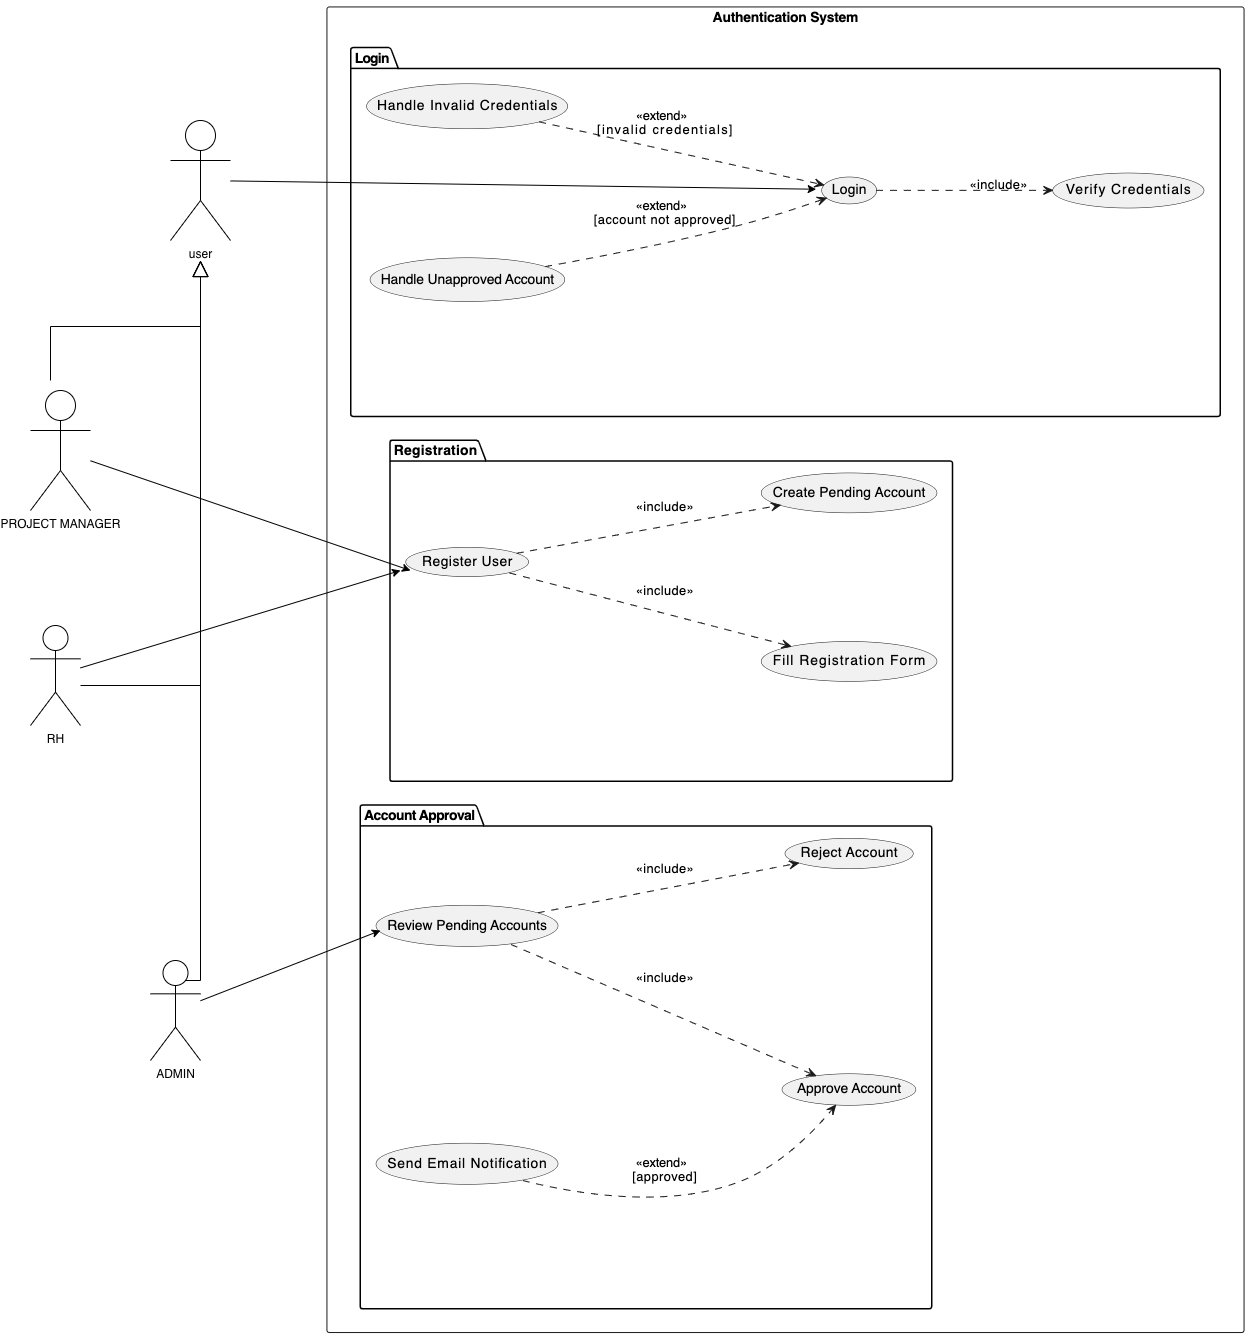
\includegraphics[width=0.96\textwidth,height=0.72\textheight,keepaspectratio]{diagrams/auth/auth-use-case-refinement.png}
}{%
    \fbox{\parbox{0.9\textwidth}{
    \centering
    \vspace{1.8cm}
    \textit{Missing file: diagrams/auth/auth-use-case-refinement.png}\\
    \textit{Insert authentication use case refinement diagram.}
    \vspace{1.8cm}
    }}
}
\end{figure}


\clearpage

\subsection{Detailed Sequence Diagrams}
For readability, each sequence diagram is presented below with its own caption and interpretation.
\textbf{Authentication flow sequence:}
\begin{enumerate}[noitemsep]
    \item Login and token issuance (Figure~\ref{fig:auth-login-flow}).
    \item Access to protected routes (Figure~\ref{fig:auth-protected-route-flow}).
    \item Token expiration and re-authentication (Figure~\ref{fig:auth-token-expiration-flow}).
    \item Logout and session invalidation (Figure~\ref{fig:auth-logout-flow}).
\end{enumerate}

\Needspace{0.62\textheight}
\textbf{Login Sequence Diagram}
Figure~\ref{fig:auth-login-flow} shows credential submission, validation, and token generation.
The user sends email and password to the authentication endpoint, where credentials and account status are checked before access is granted. If the user is an Admin, the system sends an OTP code to the admin email and waits for code validation before issuing access. When validation succeeds, the backend returns a JWT used for later API calls.

\begin{figure}[H]
\caption{Login flow showing JWT token issuance}
\label{fig:auth-login-flow}
\centering
\IfFileExists{diagrams/ch2-auth-login-flow.png}{%
    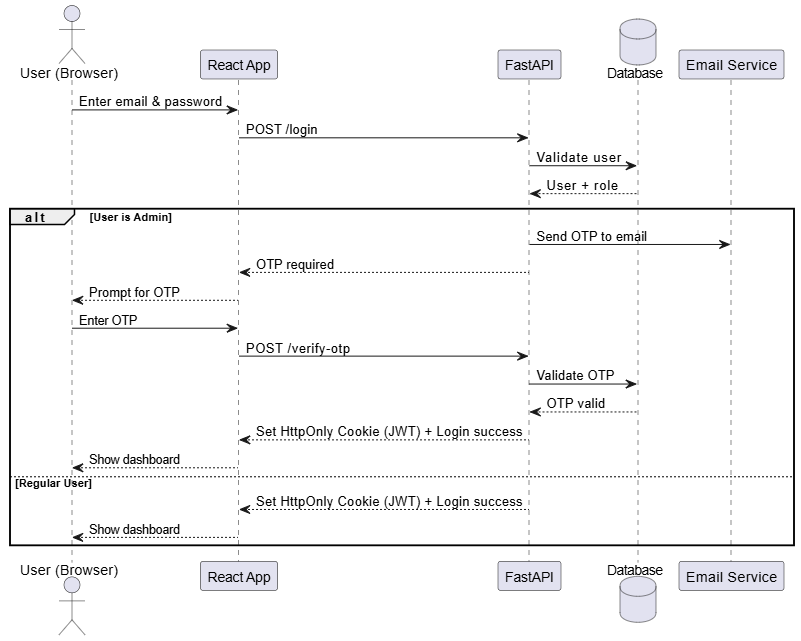
\includegraphics[width=0.94\textwidth,height=0.52\textheight,keepaspectratio]{diagrams/ch2-auth-login-flow.png}
}{%
    \fbox{\parbox{0.9\textwidth}{
    \centering
    \vspace{1.8cm}
    \textit{Missing file: diagrams/ch2-auth-login-flow.png}\\
    \textit{Insert login sequence diagram.}
    \vspace{1.8cm}
    }}
}
\end{figure}


\Needspace{0.48\textheight}
\textbf{Protected Route Access Sequence Diagram}
Figure~\ref{fig:auth-protected-route-flow} explains token and role verification before protected resources are served.
For each protected request, middleware validates token signature and expiration, then extracts user identity and role claims. The endpoint runs only if RBAC permissions allow access to the requested resource.

\begin{figure}[H]
\caption{Protected route access with JWT verification}
\label{fig:auth-protected-route-flow}
\centering
\IfFileExists{diagrams/ch2-auth-protected-route-flow.png}{%
    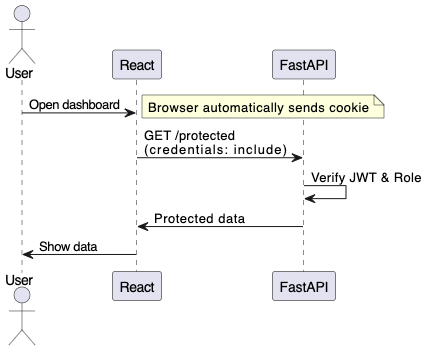
\includegraphics[width=0.94\textwidth,height=0.52\textheight,keepaspectratio]{diagrams/ch2-auth-protected-route-flow.png}
}{%
    \fbox{\parbox{0.9\textwidth}{
    \centering
    \vspace{1.8cm}
    \textit{Missing file: diagrams/ch2-auth-protected-route-flow.png}\\
    \textit{Insert protected route access sequence diagram.}
    \vspace{1.8cm}
    }}
}
\end{figure}


\Needspace{0.48\textheight}
\textbf{Token Expiration Sequence Diagram}
Figure~\ref{fig:auth-token-expiration-flow} describes session expiration and re-authentication behavior.
When the token lifetime ends, the API rejects the request with an unauthorized response and the client redirects the user to sign in again. This mechanism enforces short sessions and reduces risks linked to stale credentials.

\begin{figure}[H]
\caption{Token expiration and re-authentication flow}
\label{fig:auth-token-expiration-flow}
\centering
\IfFileExists{diagrams/ch2-auth-token-expiration-flow.png}{%
    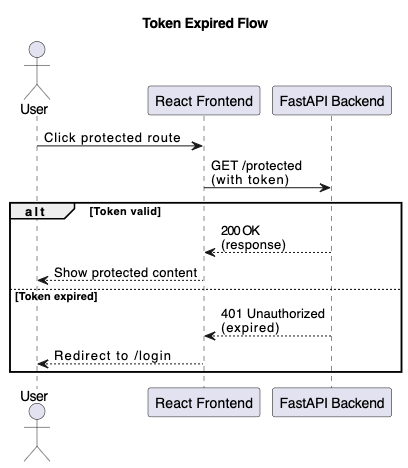
\includegraphics[width=0.94\textwidth,height=0.52\textheight,keepaspectratio]{diagrams/ch2-auth-token-expiration-flow.png}
}{%
    \fbox{\parbox{0.9\textwidth}{
    \centering
    \vspace{1.8cm}
    \textit{Missing file: diagrams/ch2-auth-token-expiration-flow.png}\\
    \textit{Insert token expiration sequence diagram.}
    \vspace{1.8cm}
    }}
}
\end{figure}


\Needspace{0.48\textheight}
\textbf{Logout Sequence Diagram}
Figure~\ref{fig:auth-logout-flow} presents controlled session termination and token invalidation.
During logout, the client clears local authentication data and stops sending the previous token in future requests. Any later access to protected routes requires a new login and a newly issued token.

\begin{figure}[H]
\caption{Logout flow with token invalidation}
\label{fig:auth-logout-flow}
\centering
\IfFileExists{diagrams/ch2-auth-logout-flow.png}{%
    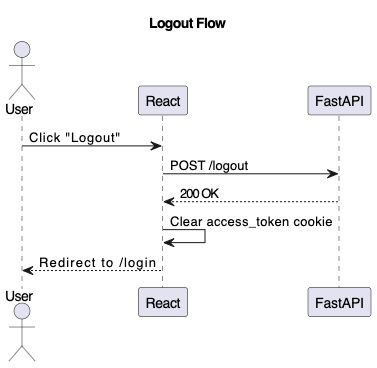
\includegraphics[width=0.94\textwidth,height=0.52\textheight,keepaspectratio]{diagrams/ch2-auth-logout-flow.png}
}{%
    \fbox{\parbox{0.9\textwidth}{
    \centering
    \vspace{1.8cm}
    \textit{Missing file: diagrams/ch2-auth-logout-flow.png}\\
    \textit{Insert logout sequence diagram.}
    \vspace{1.8cm}
    }}
}
\end{figure}


\section{Sprint Realization}
\subsection{Authentication Interface}
The implemented authentication interface includes the login view, credential validation feedback, and the OTP verification step for Admin users.

Figure~\ref{fig:auth-login-ui} shows email/password authentication, user feedback on invalid credentials, and the Admin OTP verification step.

\begin{figure}[H]
\caption{Login interface of the application}
\label{fig:auth-login-ui}
\centering
\IfFileExists{assets/auth/auth-login-screen.png}{%
    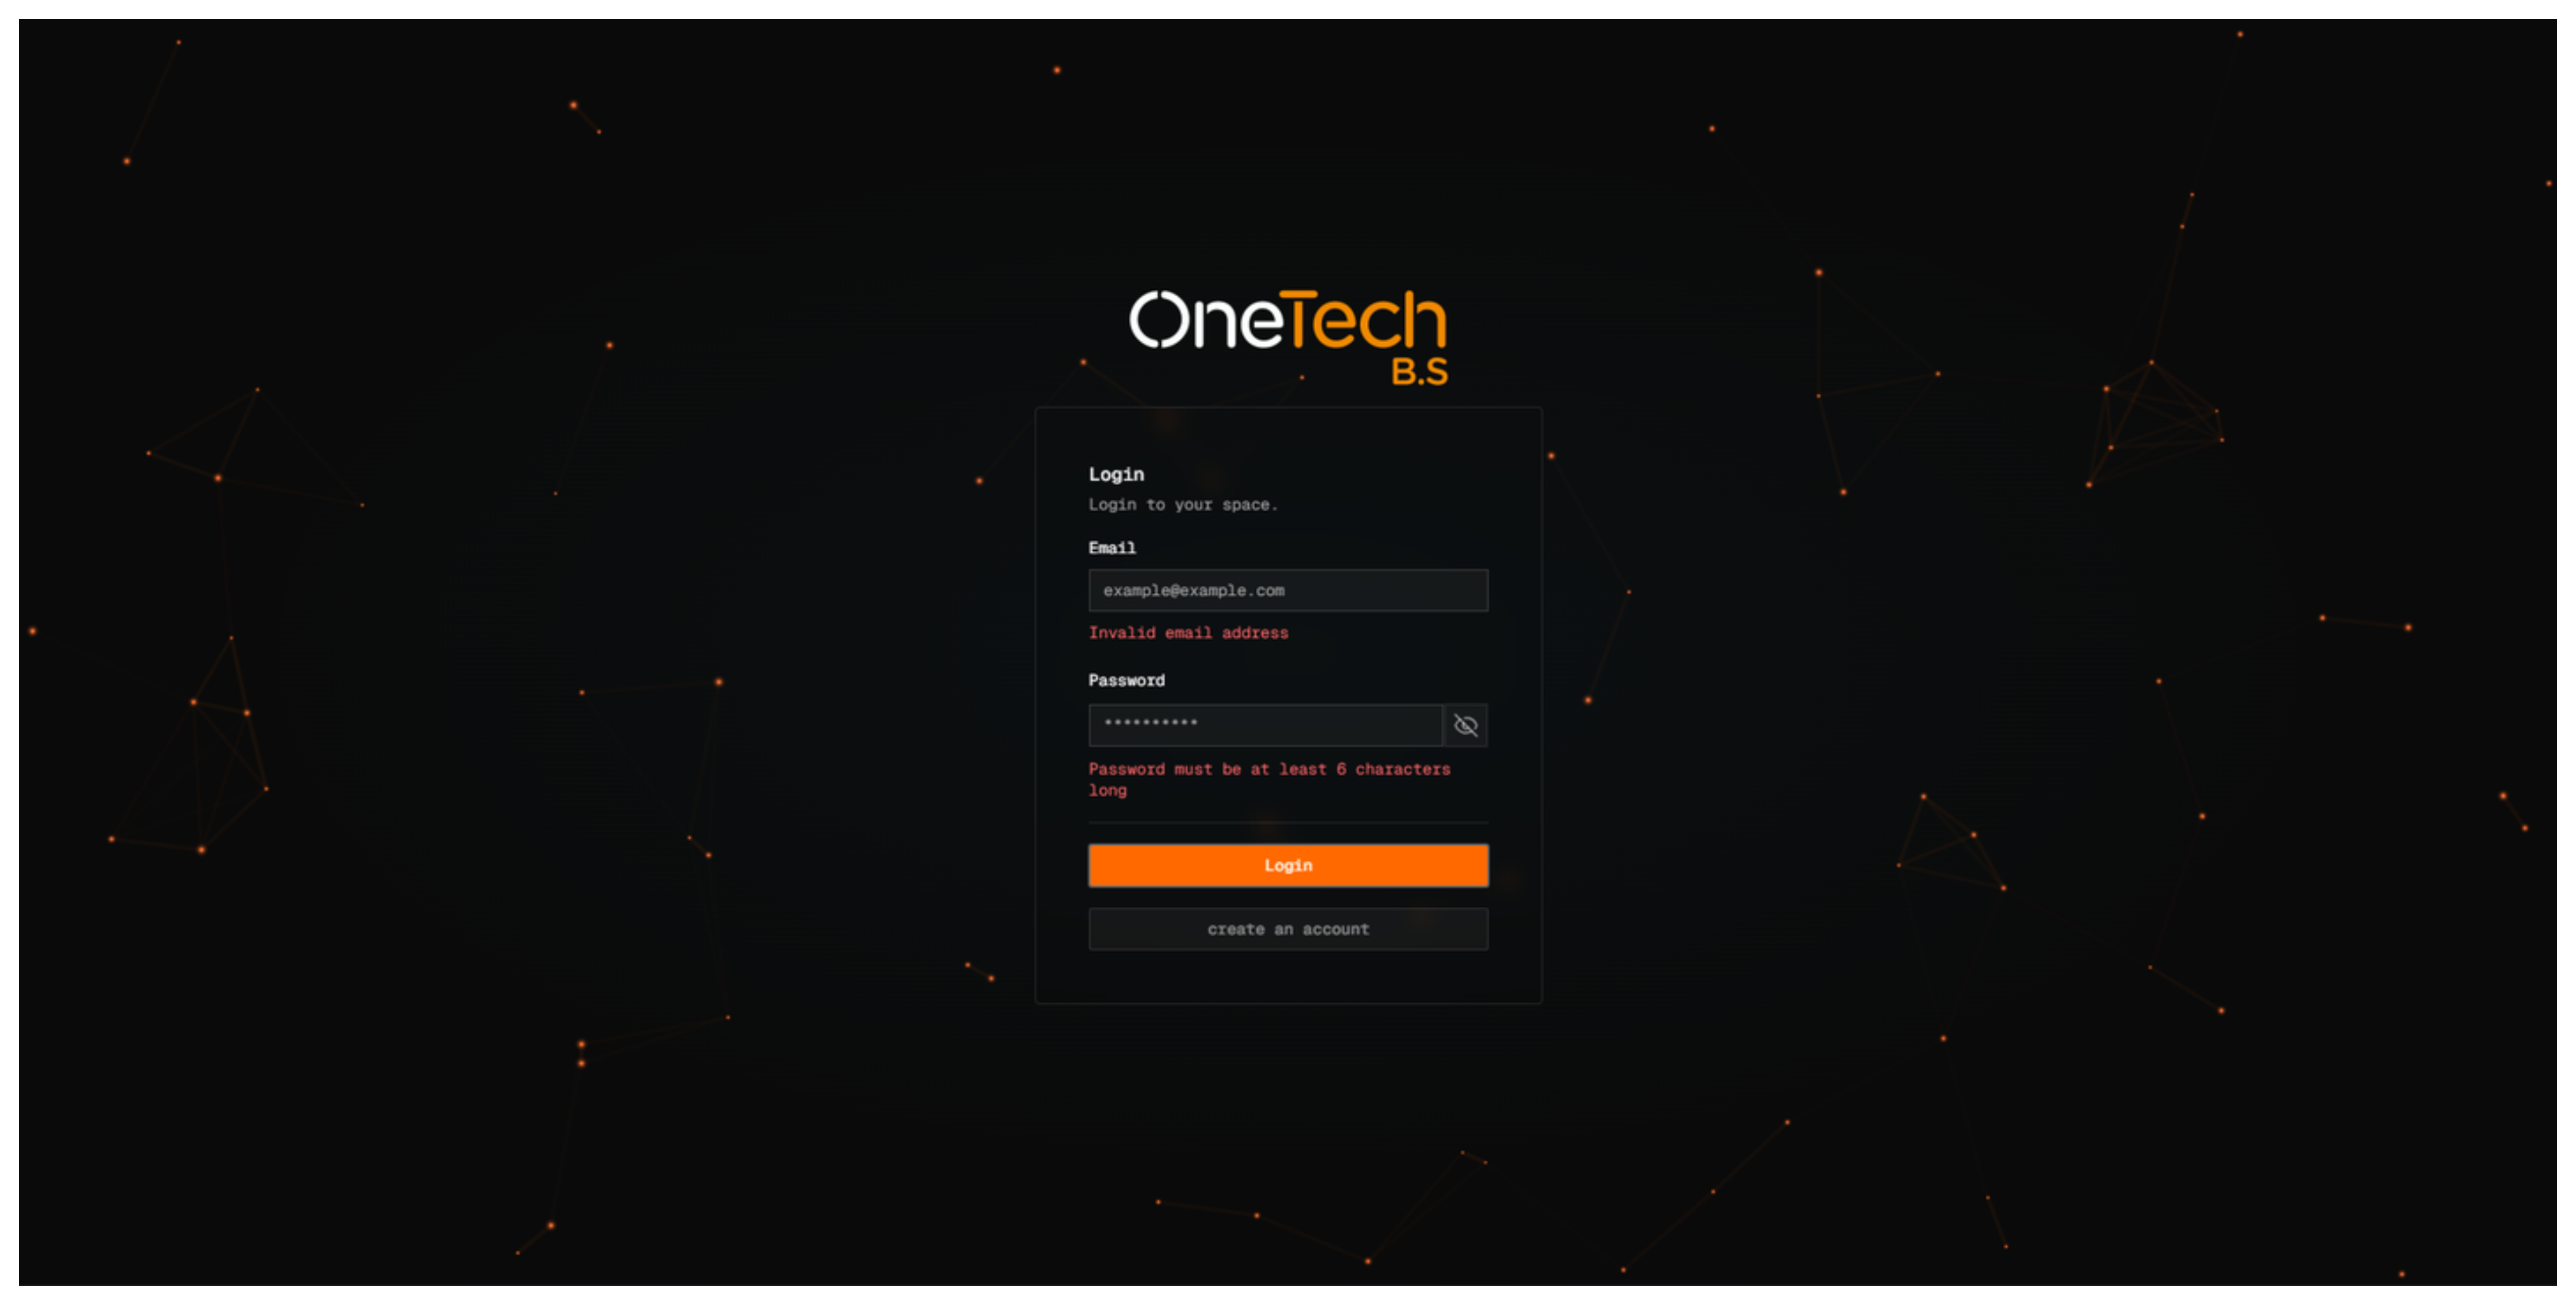
\includegraphics[width=0.92\textwidth,height=0.48\textheight,keepaspectratio]{assets/auth/auth-login-screen.png}
}{%
    \fbox{\parbox{0.9\textwidth}{
    \centering
    \vspace{1.6cm}
    \textit{Missing file: assets/auth/auth-login-screen.png}\\
    \textit{Insert screenshot of the login page interface.}
    \vspace{1.6cm}
    }}
}
\end{figure}


\subsection{Admin OTP Verification Interface}
After entering valid login credentials, the Admin is asked to enter the OTP code sent to their email.

Figure~\ref{fig:auth-admin-otp-ui} presents the extra verification step where the Admin enters the code received by email before access is granted.

\begin{figure}[H]
\caption{Administrator OTP verification interface}
\label{fig:auth-admin-otp-ui}
\centering
\IfFileExists{assets/auth/admin-otp-screen.png}{%
    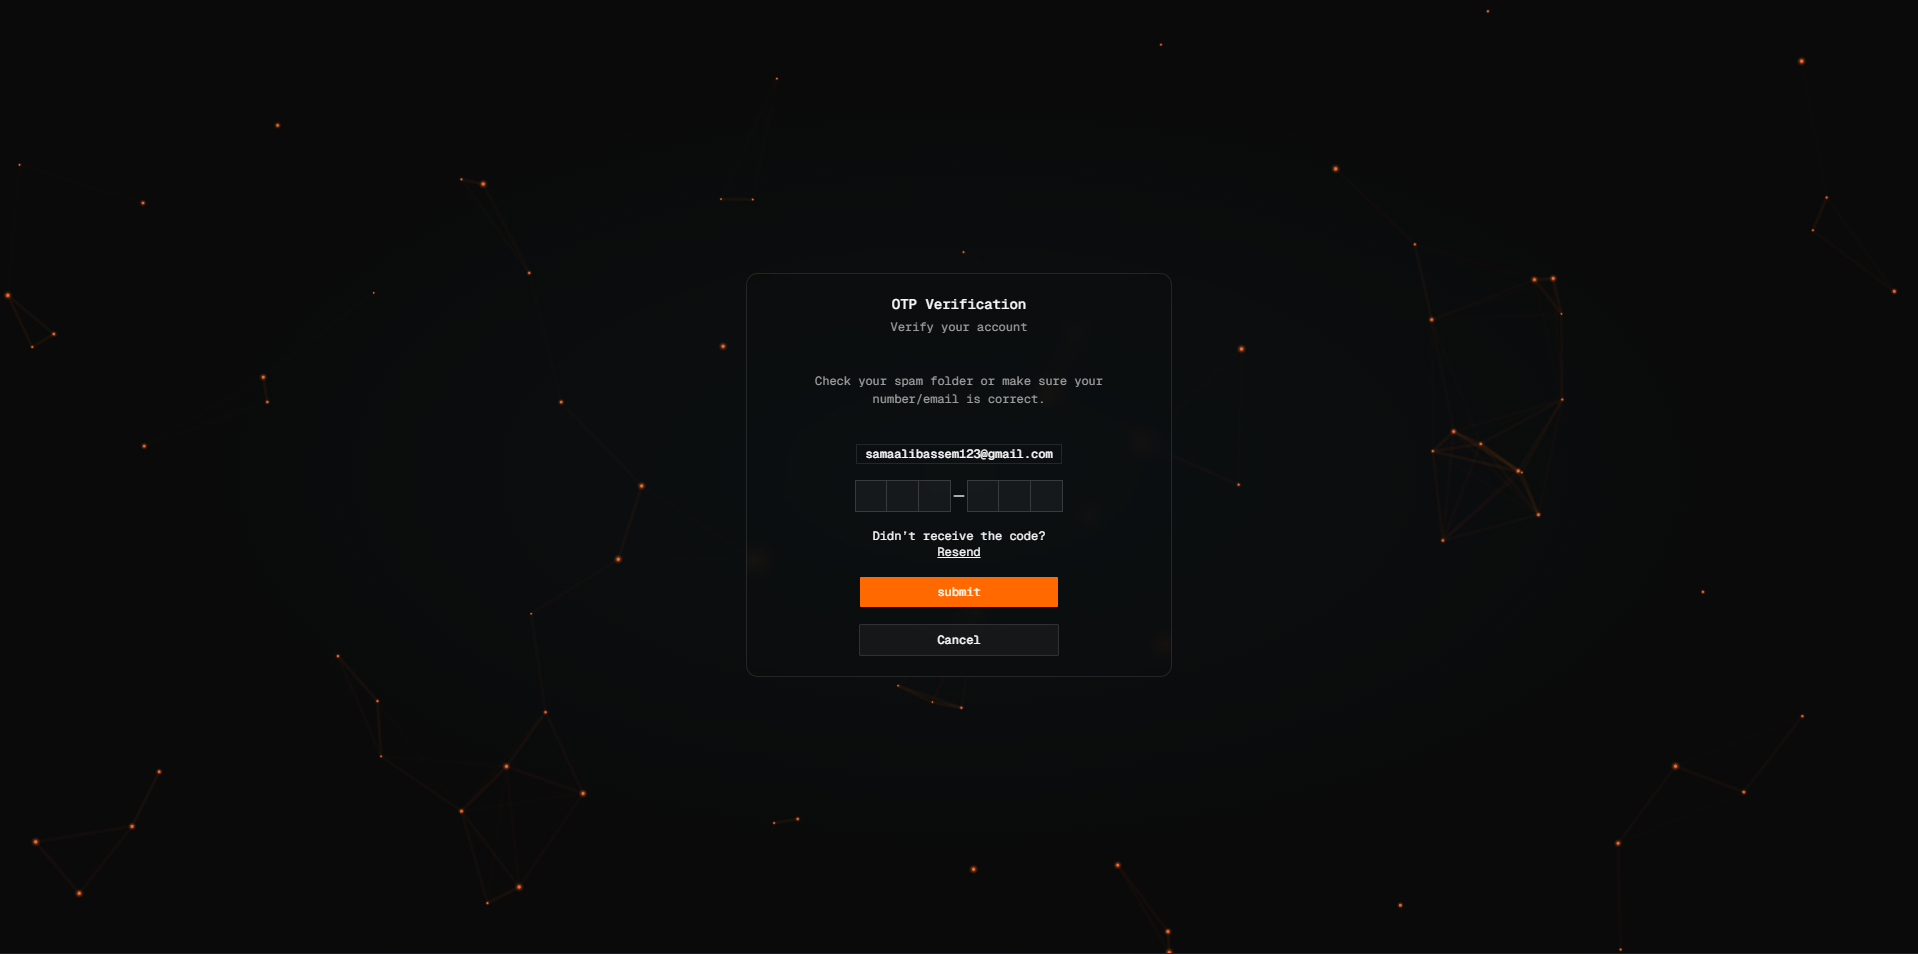
\includegraphics[width=0.92\textwidth,height=0.48\textheight,keepaspectratio]{assets/auth/admin-otp-screen.png}
}{%
    \fbox{\parbox{0.9\textwidth}{
    \centering
    \vspace{1.6cm}
    \textit{Missing file: assets/auth/admin-otp-screen.png}\\
    \textit{Insert screenshot of the Admin OTP verification page.}
    \vspace{1.6cm}
    }}
}
\end{figure}


\subsection{Registration Interface}
The registration interface allows account creation for operational roles before administrator validation.

Figure~\ref{fig:auth-register-ui} presents account creation for HR and Project Manager roles with pending approval status.

\begin{figure}[H]
\caption{User registration interface}
\label{fig:auth-register-ui}
\centering
\IfFileExists{assets/auth/auth-register-screen.png}{%
    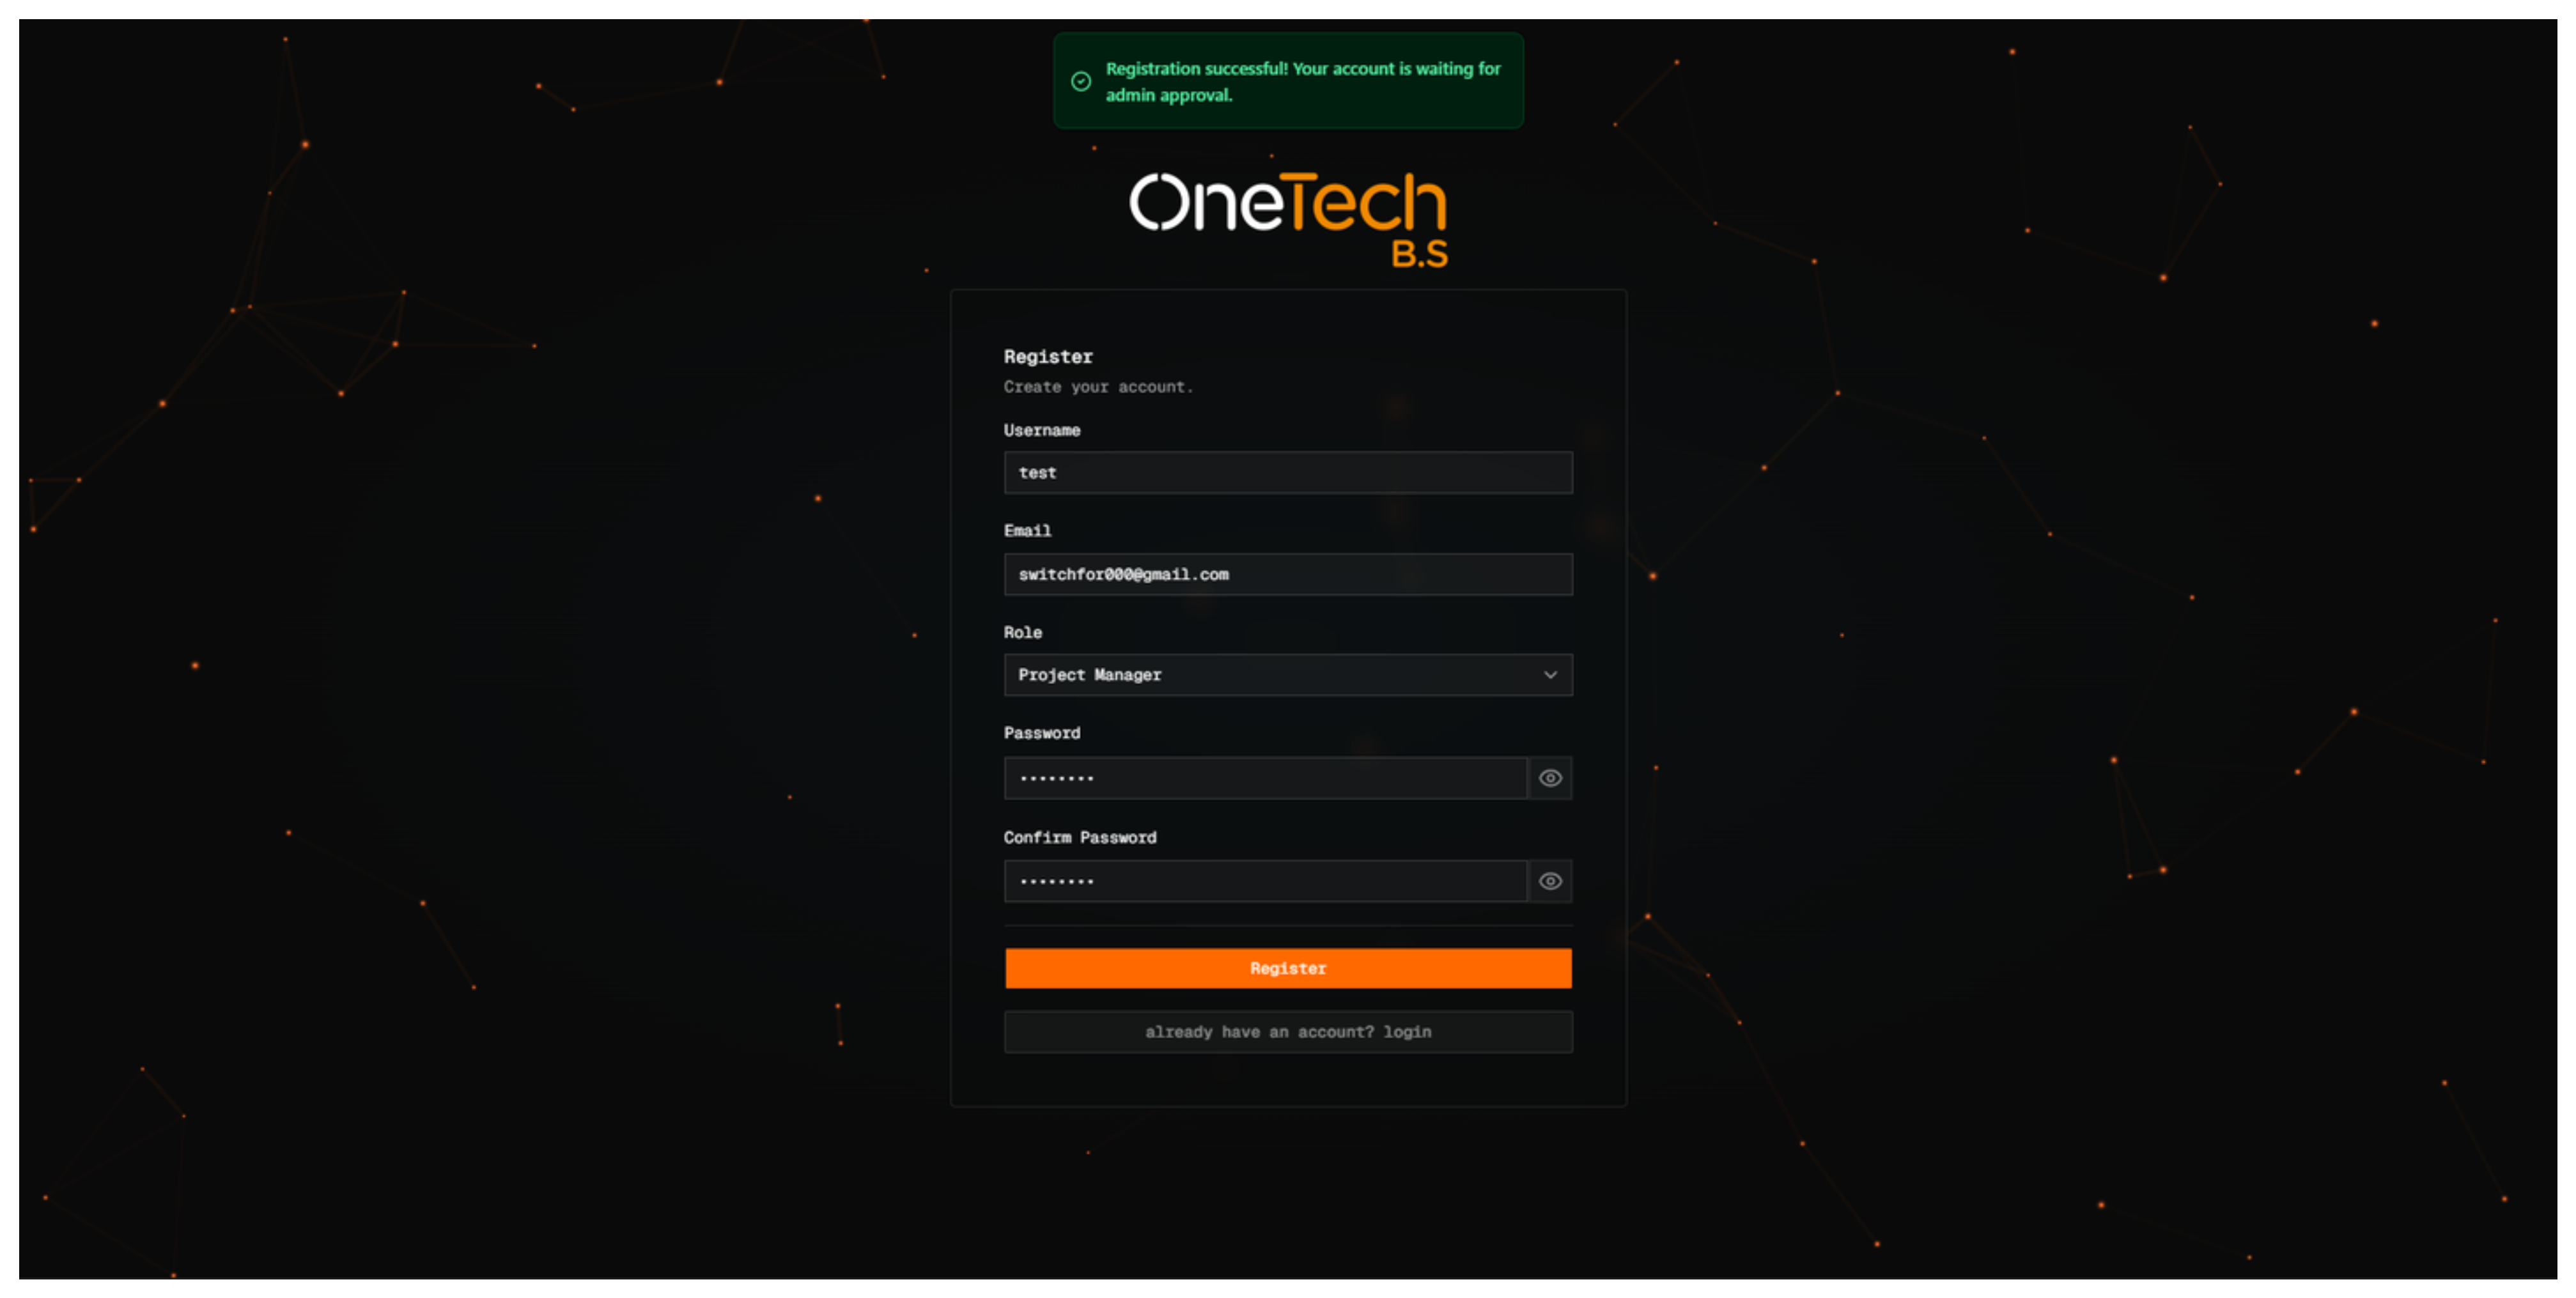
\includegraphics[width=0.92\textwidth,height=0.48\textheight,keepaspectratio]{assets/auth/auth-register-screen.png}
}{%
    \fbox{\parbox{0.9\textwidth}{
    \centering
    \vspace{1.6cm}
    \textit{Missing file: assets/auth/auth-register-screen.png}\\
    \textit{Insert screenshot of the registration page interface.}
    \vspace{1.6cm}
    }}
}
\end{figure}


\subsection{Administrator Account Approval Interface}
After registration, accounts remain pending until administrator approval.

Figure~\ref{fig:admin-approve-account-ui} shows the pending-user list and approval/rejection actions.

\begin{figure}[H]
\caption{Administrator page for account approval}
\label{fig:admin-approve-account-ui}
\centering
\IfFileExists{assets/auth/admin-approve-account.png}{%
    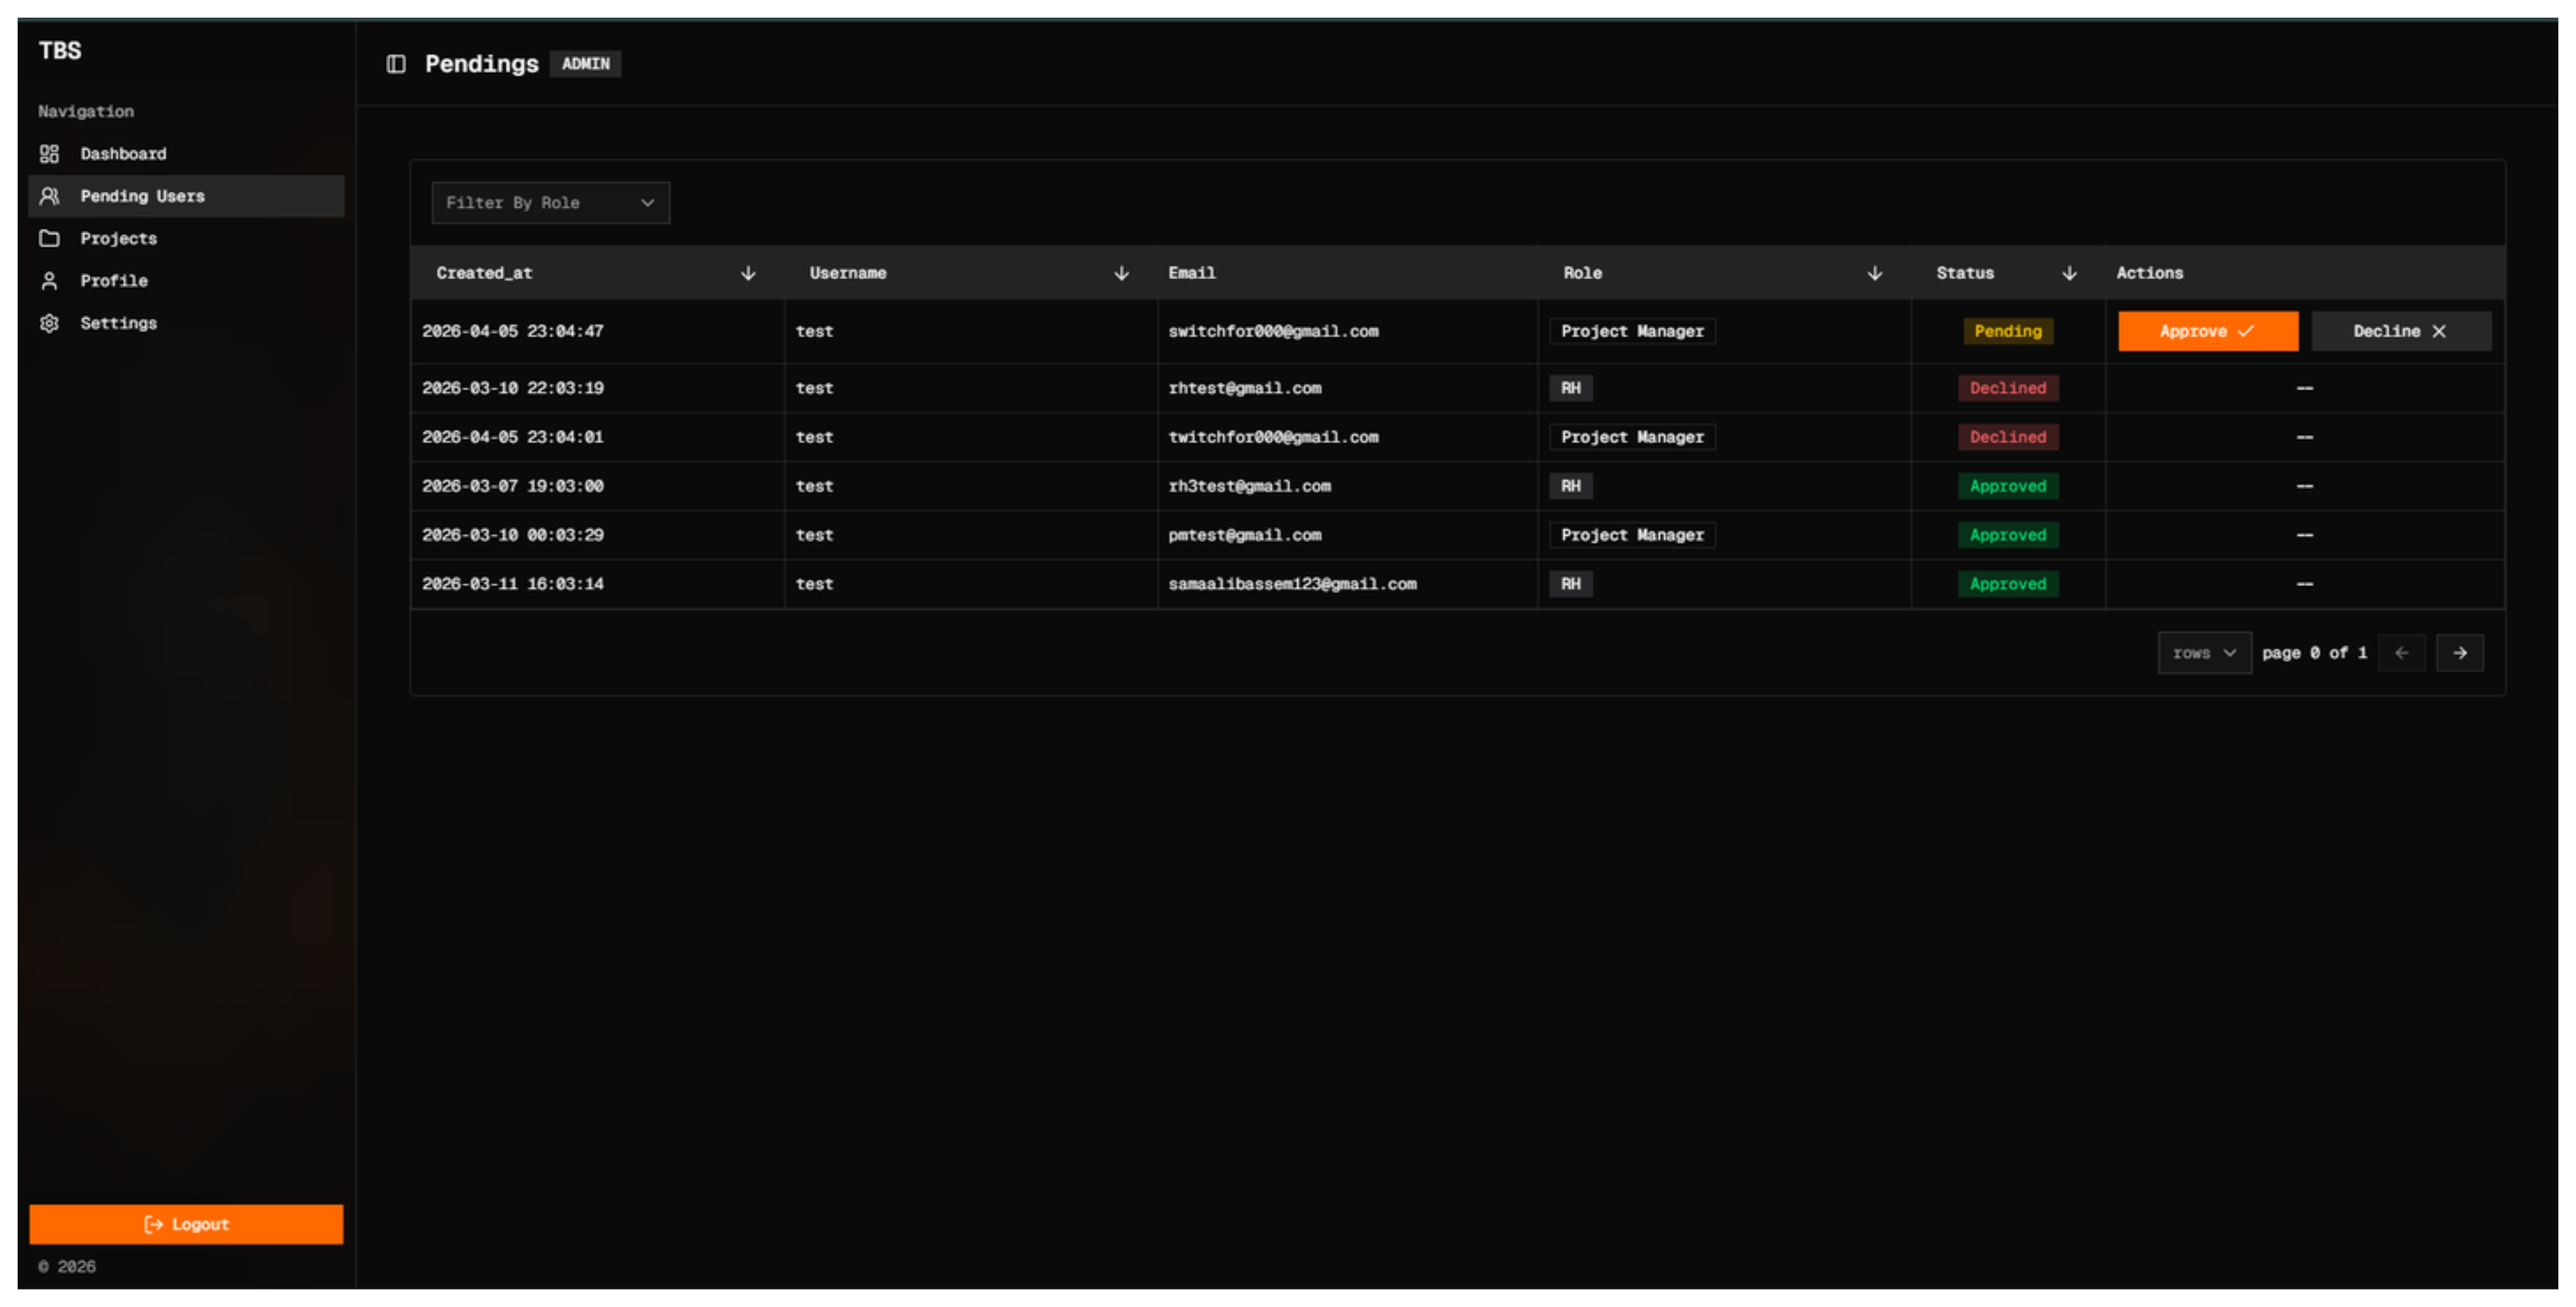
\includegraphics[width=0.92\textwidth,height=0.48\textheight,keepaspectratio]{assets/auth/admin-approve-account.png}
}{%
    \fbox{\parbox{0.9\textwidth}{
    \centering
    \vspace{1.6cm}
    \textit{Missing file: assets/auth/admin-approve-account.png}\\
    \textit{Insert screenshot of the admin approval interface.}
    \vspace{1.6cm}
    }}
}
\end{figure}


\subsection{Approval Email Notification}
When an account is approved, the system sends an automatic activation email.

Figure~\ref{fig:account-approval-email} confirms automated communication of account activation.

\begin{figure}[H]
\caption{Account approval email notification}
\label{fig:account-approval-email}
\centering
\IfFileExists{assets/auth/account-approval-email.png}{%
    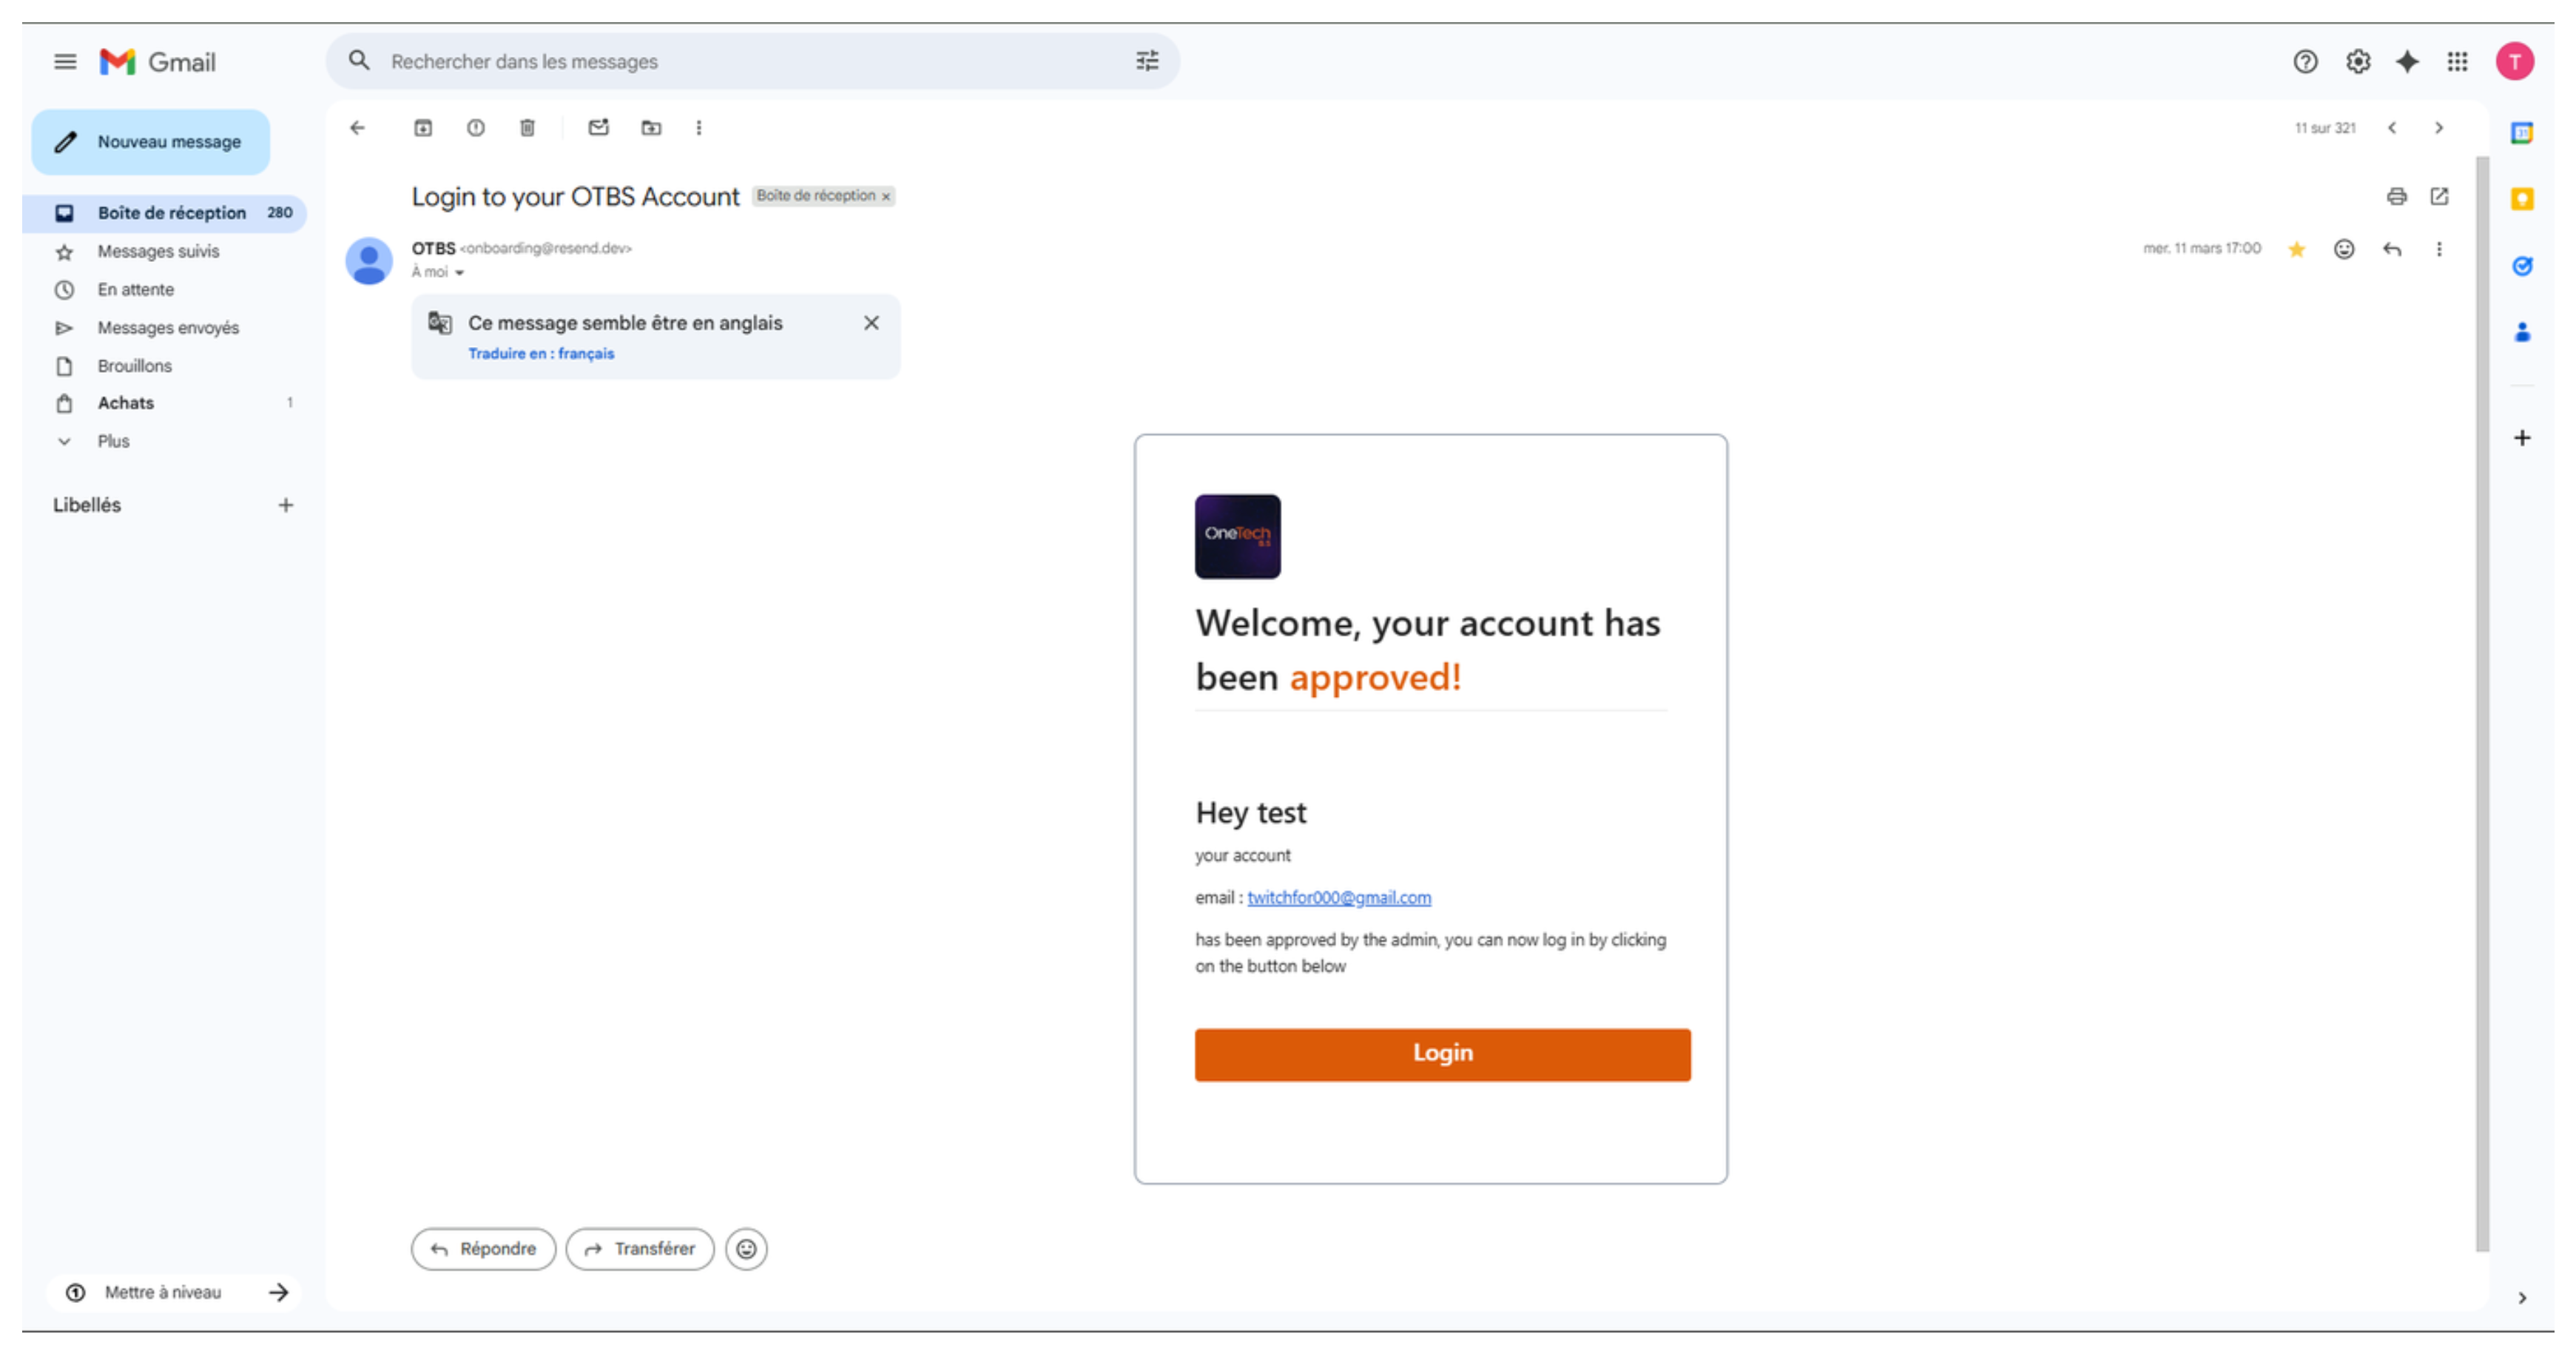
\includegraphics[width=0.92\textwidth,height=0.48\textheight,keepaspectratio]{assets/auth/account-approval-email.png}
}{%
    \fbox{\parbox{0.9\textwidth}{
    \centering
    \vspace{1.6cm}
    \textit{Missing file: assets/auth/account-approval-email.png}\\
    \textit{Insert screenshot of the account approval email.}
    \vspace{1.6cm}
    }}
}
\end{figure}


\subsection{Error Handling Scenarios}
The implemented logic provides explicit user feedback in critical cases:
\begin{itemize}[noitemsep]
    \item Incorrect email/password: the system displays an authentication error.
    \item Correct credentials with pending account: access is denied with an approval-status message.
    \item Admin login with invalid or expired OTP: access is denied until the correct code is entered.
\end{itemize}

\section{Security Considerations}
The following security controls were applied in the authentication module:

\begin{center}
\renewcommand{\arraystretch}{1.2}
\begin{tabular}{|l|>{\raggedright\arraybackslash}p{9.8cm}|}
\hline
\textbf{Control} & \textbf{Description} \\
\hline
Password hashing & Passwords are stored as hashes (e.g., bcrypt) rather than plaintext. \\
\hline
Input validation & Form inputs are validated to prevent invalid or malformed authentication requests. \\
\hline
Secure error handling & Authentication errors do not expose sensitive system details. \\
\hline
RBAC enforcement & Access to protected resources depends on verified user role permissions. \\
\hline
Approval-gated access & Users cannot access business modules unless account status is approved by the administrator. \\
\hline
Admin OTP verification & Admin users must validate a one-time password sent by email before login is completed. \\
\hline
\end{tabular}
\end{center}

\section{Conclusion}
The authentication module ensures secure and controlled access to the application. With administrator approval, automatic email notification, and OTP verification for Admin users, the system adds an extra layer of protection for sensitive access.
